\documentclass{standalone}
\usepackage{tikz}
\usepackage{ctex,siunitx,ninecolors}
\setCJKmainfont{Noto Serif CJK SC}
\usepackage{tkz-euclide}
\usepackage{amsmath}
\usetikzlibrary{patterns, calc}
\usetikzlibrary {decorations.pathmorphing, decorations.pathreplacing, decorations.shapes}
\begin{document}
\small
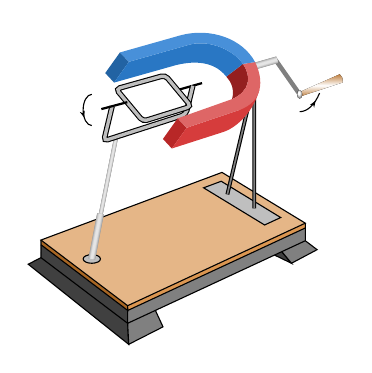
\begin{tikzpicture}[>=latex, scale=1.1]
  % \useasboundingbox(0.9,0)rectangle(5.1,5);
  \draw[fill=darkgray](0.213,1.115)--(0.066,1.039)--(1.226,0.114)--(1.214,0.357)(2.909,1.145)--(3.105,1.050)--(2.994,1.184)(0.214,1.263)--(0.213,1.115)--(1.214,0.357)--(1.214,0.506);
  \draw[fill=gray](1.534,0.506)--(1.622,0.316)--(1.226,0.114)--(1.214,0.357)
  (3.265,1.310)--(3.401,1.207)--(3.105,1.050)--(2.994,1.184)(3.266,1.458)--(3.265,1.310)--(1.214,0.357)--(1.214,0.506);
  \draw[fill=brown5](1.214,0.560)--(1.215,0.505)--(0.214,1.263)--(0.213,1.318);
  \draw[fill=brown7](1.214,0.560)--(1.215,0.505)--(3.266,1.458)--(3.265,1.513);
  \draw[fill=brown8](0.213,1.318)--(2.303,2.099)--(3.265,1.513)--(1.214,0.560)--cycle;
  \draw[fill=lightgray](2.091,1.921)--(2.795,1.492)--(2.981,1.578)--(2.294,1.997)--cycle;
  \draw[double=gray](2.675,1.685)--(2.675,3.150)--(2.365,1.845);
  \draw[fill=lightgray](0.8,1.1)ellipse(0.1 and 0.05);
  \foreach \x in {80,70,...,20}
  {
    \draw[line width={1.5*sin(\x)},gray!\x](0.8,1.1)--(1.08,2.5);
  }
  \draw[ultra thick,gray](3.2,3.0)--(2.92,3.4);
  \foreach \x in {80,70,...,20}
  {
    \draw[line width={2.5*sin(\x)},gray!\x](0.8,1.1)--(0.9,1.62);
    \draw[line width={2.5*sin(\x)},gray!\x](2.59,3.3)--(2.94,3.4);
  }
  \draw[thick](1.79,3.05)--(2.073,3.13);
  \draw[double=lightgray,rounded corners=0.5mm,double distance=1.2pt](1.034,2.862)--(0.939,2.463)--(1.886,2.769)--(1.966,3.100);
  \draw[double=lightgray,rounded corners=0.5mm,double distance=1.2pt](1.946,2.862)--(1.647,3.221)--(1.080,3.062)--(1.391,2.689)--cycle;
  \draw[thick](1.21,2.91)--(0.91,2.83);
  \fill[red4](1.791,2.723)--(1.621,2.485)--(1.724,2.375)--(1.895,2.614)--cycle;
  \fill[red3](2.353,3.205)..controls(2.407,3.147)and(2.451,3.058)..
  (2.419,2.945)..controls(2.628,3.038)and(2.647,3.206)..(2.544,3.351)--cycle;
  \fill[red5](1.895,2.614)--(1.724,2.375)--(2.328,2.569)..controls(2.427,2.603)and(2.645,2.744)..(2.734,3.049)--(2.508,2.821)--cycle;
  \fill[red6](2.544,3.351)..controls(2.647,3.206)and(2.628,3.038)..(2.419,2.945)--(1.791,2.723)--(1.895,2.614)--(2.508,2.821)..controls(2.777,2.921)and(2.788,3.162)..(2.685,3.373)--cycle;
  \fill[azure4](1.125,3.484)--(0.955,3.246)--(1.057,3.136)--(1.228,3.376)--cycle;
  \fill[azure5](1.228,3.376)--(1.940,3.577)..controls(2.161,3.631)and(2.437,3.512)..(2.544,3.351)--(2.353,3.205)..controls(2.276,3.303)and(2.116,3.423)..(1.769,3.337)--(1.057,3.136)--cycle;
  \fill[azure6](1.940,3.577)..controls(2.161,3.631)and(2.437,3.512)..(2.544,3.351)--(2.685,3.373)..controls(2.538,3.646)and(2.173,3.770)..(1.836,3.685)--(1.125,3.484)--(1.228,3.376)--cycle;
  \fill[top color=brown,bottom color=brown,middle color=white](3.186,3.021)--(3.662,3.232)to[bend left](3.698,3.138)--(3.204,2.975)to[bend left ](3.186,3.021)--cycle;
  \fill[ball color=white](3.2,3.0)ellipse(0.03 and 0.05);
  \draw[postaction={decorate},decoration={markings,mark=at position 0.7 with {\arrow{Stealth[scale=0.5]}}}](3.2,2.8)arc(270:320: 0.3 and 0.6);
  \draw[postaction={decorate},decoration={markings,mark=at position 0.7 with {\arrow{Stealth[scale=0.5]}}}](0.8,3.0)arc(90:270: 0.1 and 0.18);
\end{tikzpicture}
\end{document}